\section{Introduction: Axioms of Quantum Mechanics}
\begin{itemize}
	\item Also called postulates.
	\item Typically four axioms:
		\begin{enumerate}[label=\arabic*.]
			\item Quantum states \& superposition
			\item Unitary Evolution: deterministic
			\item Measurements: introduces statistical nature to quantum behavior
			\item Observables: quantities we can measure in the real world 
		\end{enumerate}
\end{itemize}

\subsection{Quantum States}
\begin{itemize}
	\item A quantum state is denoted by \( \ket{\psi} \). It's a vector in a complex-valued vector space, with a
		particular inner product structure. This combination of the vector space with the inner product structure 
		is called a Hilbert space, denoted by \( \mathcal H \). 
	\item Vectors in \( \mathcal H \) are denoted by \textit{kets} \( \ket{v} \), and because it's a vector space 
		(hence it's linear), we can make other vectors by adding together two vectors: \( \ket{w} = \ket{u} + 
		\ket{v}\). 

		We also have a null vector \( \ket{0} = \ket{u} - \ket{u} \). 
	\item Linearly independent vectors: 
		\[
		a_1\ket{u_1} + a_2\ket{u_2} + \cdots + a_n\ket{u_n} = 0
		\] 
		if the only solution to this is to set \( a_1, a_2, \dots, a_n \) to 0, then the set of vectors 
		\( \ket{u_1}, \ket{u_2}, \dots, \ket{u_n} \) is linearly independent. 
		
		\comment{We will only work with finite dimensional vector spaces, for the sake of quantum information}
	\item If the set of vectors \( \{\ket{u_i}\}  \) spans the space, then they are referred to as a basis. This 
		means that any vector \( \ket{w} \) can be written as a linear combination of some \( \ket{u_i} \) :
		\[
			\ket{w} = \sum_i a_i \ket{u_i} 
		\]
		It can also be represented as a column vector of \( n \) values:
		 \[
		\ket{w} = \begin{bmatrix} a_1 \\ \vdots \\ a_n \end{bmatrix} 
		\] 
	\item An example where \( n = 2 \), is \textit{spin projection}, which has two possible values: \( \pm 
		\hbar / 2\). In this case, the general state \( \ket{\psi}  \) can be written as 
		\( \ket{\psi} = a_1\ket{+\hbar / 2} + a_2\ket{-\hbar / 2} \). 
		
		We'll be dealing with mostly two-state systems in this class, and any other two-state system that we choose 
		is sometimes called "pseudo-spin" since the math is nearly identical. 
	\item In all cases, we should have \( \sum_i |a_i|^2 = 1 \); we call the states that follow this behavior 
		(and they should) to be \textbf{normalized to 1}. 
\end{itemize}
\subsection{Inner Product}
\begin{itemize}
	\item Given \( \ket{w} = \sum_i a_i \ket{u_i} \) and \( v = \sum_i b_i \ket{u_i} \), then the complex-valued 
		inner product \( \braket*{v}{w} = \sum_i b_i^* a_i\). It can be real-valued, but in general it's considered
		complex. 

		This gives a way for us to talk about how far apart two vectors are from one another, similar to a dot
		product. 
	\item If the inner product is 0 and our vectors are not the zero vector themselves, then we call these two vectors 
		\textbf{orthogonal}.
	\item An \textbf{orthonormal basis} is one where all the vectors are orthogonal, and also normalized to 1. In other
		words, we have \( \braket*{u_i}{u_j} = \delta_{ij} \), where \( \delta_{ij} \) is the Kronecker delta. 
	\item So what is \( \bra{u} \)? \( \bra u \) lives in the \textit{dual space}, and is defined as follows: if 
		\( \ket{w} = \sum_i a_i \ket{u_i} \), then \( \bra{w} = \sum_i a_i^* \bra{u_i} \). 

		So if \(  \ket{w} \) is represented as a column vector (earlier), then \( \bra{w} \) is represented as a 
		row vector:
		\[
			\bra{w} = \begin{bmatrix} a_1^* & \hdots & a_n^* \end{bmatrix} = {w^\top}^* = w^{\dagger}
		\] 
	\item The properties of the inner product:
		\begin{itemize}
			\item \( \braket*{u}{v} = \braket*{v}{u}^* \) 
			\item Antilinearity: \( \braket*{u}{av} = a\braket*{u}{v} \), but
				\( \braket*{au}{v} = a^*\braket*{u}{v} \). 
			\item Norm of \( \ket{v} \) : \( \braket*{v}{v} = \|v\|^2 \). Hence, \( \|v\| = \sqrt{\braket*{v}{v}}  \).
		\end{itemize}
	\item Conventionally, although we denote \( \ket{w} = \sum_i^{n - 1}a_i \ket{u_i} \), we generally deal with 
		\( n = 2 \), so we have \( \ket{0} \) and \( \ket{1} \) as our states. This is called the \textbf{computational
		basis}.
\end{itemize}
\subsection{Geometric Interpretation}
\begin{itemize}
	\item For \( n = 2 \), there is a nice geometric interpretation called the \textbf{Bloch sphere}:
		\begin{center}
			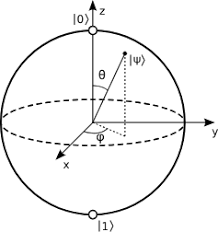
\includegraphics[scale=0.8]{bloch-sphere.png}
		\end{center}
		The sphere has radius 1, and all points on the sphere represent quantum states. A general state 
		\( \ket{\psi} \) is written as 
		\[
		\ket{\psi} = e^{i\gamma}\left[ \cos \frac{\theta}{2}\ket{0} + e^{i\phi}\sin \frac{\theta}{2}\ket{1} \right] = 
		\alpha\ket{0} + \beta\ket{1}
		\] 
		If we want our state to be normalized, then we want \( \|\alpha\|^2 + \|\beta\|^2 = 1 \).  
	\item There are also other orthonormal bases we can choose:
		\begin{itemize}
			\item x-basis: \( \ket{+x} = \frac{1}{\sqrt{2} }(\ket{0} + \ket{1} \) , \( \ket{-x} = \frac{1}{\sqrt{2} }
				(\ket{0} - \ket{1})\). 
			\item y-basis: \( \ket{+y}= \frac{1}{\sqrt{2} }(\ket{0} + i\ket{1} \), and \( \ket{-y} = 
				\frac{1}{\sqrt{2} }(\ket{0} - i\ket{1})\).
		\end{itemize}
\end{itemize}
\subsection{Unitary Evolution}
\begin{itemize}
	\item All equations we'll deal with are relations in \( \mathcal H \), and these operations form a group 
		called SU(2). This is called the \textit{Special unitary group}.
	\item This unitary transformation takes our vectors \( \ket{0} \) and \( \ket{1} \) and does the following:
		\begin{align*}
			\ket{0} &\overset{U}{\longrightarrow} a\ket{0} + b\ket{1}\\
			\ket{1} &\overset{U}{\longrightarrow} c\ket{0} + d\ket{1}
		\end{align*}
		In this case, we can write \( U \) as a 2x2 matrix:
		\[
			U = \begin{pmatrix} a & c\\ b& d \end{pmatrix} \ 
			U^\dagger = \begin{pmatrix} a^* & b^*\\c^* & d^* \end{pmatrix} 
		\] 
		Recall that \( U^{\dagger} \) is the conjugate transpose. If \( U \) is a unitary operator, then 
		\( U\dagger U = I = U U^{\dagger}\). This implies that \( U\dagger = U^{-1} \) 
	\item On a qubit, we will apply many gates throughout this semester. Some of these are listed below:
		\begin{itemize}
			\item X-gate: \( X = \begin{pmatrix} 0 & 1 \\ 1& 0 \end{pmatrix}  \) 
			\item Z-gate: \( Z = \begin{pmatrix} 1 & 0 \\ 0 & -1 \end{pmatrix}  \) 
			\item Hadamard gate: \( H = \frac{1}{\sqrt{2} }\begin{pmatrix} 1&1\\1&-1 \end{pmatrix}  \)
		\end{itemize}
		All of these operations can be interpreted as a series of rotations on the Bloch sphere.
\end{itemize}
\subsection{Observables}
\begin{itemize}
	\item An operator \( A \), and its Hermitian conjugate is denoted by \( A^{\dagger} = (A^{\top})^{*} \).
	\item In QM, Hermitian operators are related to real observables we can measure in the lab, and because they are 
		measurable, they must have real eigenvalues.  
	\item They will also have mutually orthogonal eigenvectors. 
	\item As an example, the  \( X \) gate is Hermitian, with eigenvectors of \( \ket{+x} \) and \( \ket{-x} \). This 
		is also sometimes called the Hadamard basis, because acting the Hadamard gate on \( \ket{0} \) gives us 
		\( \ket{+x} \), and acting it on \( \ket{1} \) gives \( \ket{-x} \).  
\end{itemize}

